%describe the methodology background or domain background. Imagine a non-expert will read your paper and what he/she needs to know in order to follow your work. 
%Describe the background of your work (if applied). For instance, if you expect readers understand forking behaviors of GitHub and you are afraid that some of them do not have the background knolwedge, you can describe the background here. If you believe that majority of your audience understand the context. You don't need a background section.
In this section, we provide a more in-depth description of dependency-relationships, semantic versioning, and Greenkeeper.
% Dependency relationships
~\subsection{Dependency Relationships}
\label{sec:background.dependencies}
Software dependency relationships allow a client package to reuse a certain version of a provider package stored in online package distributions. There are over 1.6 million packages available on npm alone\footnote{https://libraries.io/npm}. These provider packages are constantly evolving, with newly added features and patches that fix bugs in older versions. Additionally, the availability of such a huge amount of reusable packages facilitates software development and evolution. However, dependency relationships can also cause problems, such as software becoming out of date with respect to more recent package releases, or, if the packages are kept up-do-date, there is a risk that the new version will break existing functionality, so developers may resort to version pinning their dependencies or other less-than-ideal solutions \cite{2019CogoDowngrades} \cite{2017_Kula_DoDevsUpdateTheirDependencys}.
% Semantic Versioning and Dependency Constraints
~\subsection{Semantic Versioning and Dependency Constraints}
\label{sec:background.semver}
With many software packages being created and updated every day, it is important to standardize the way of versioning and keeping track of package releases and dependencies. Semantic Versioning, referred as \textit{semver}, has become a popular policy for communicating the kinds of changes made to a software package. It allows dependent software packages to be informed about possible “breaking changes”. A semver-compatible version is a version number composed of a major, minor and patch number. The version numbers allow to order package releases. For example, 1.2.3 occurs before 1.2.10 (higher patch version), which occurs before 1.3.0 (higher minor version), which occurs before 2.1.0 (higher major version). Backward incompatible updates should increment the major version, updates respecting the API but adding new functionalities should increment the minor version, while simple bug fixes should increment the patch version. Unfortunately, the semantic versioning policy is not always respected by package maintainers.
\par
\textbf{npm} recommends software packages to follow a specific flavor of semantic versioning\footnote{https://docs.npmjs.com/misc/semver}. Package releases specify their version number in the metadata stored in a json file\footnote{https://docs.npmjs.com/files/package.json}, and use dependency constraints to specify the version ranges of other packages they depend upon. These constraints are built from a set of operators that specify versions that satisfy the range. Table \ref{tab:semver} summarizes the types of dependency constraints for npm, their interpretation and an example of each constraint type.
\begin{table*}[h]
    \begin{center}
    \begin{tabular}{ c|c|c|c } 
         \textbf{Constraint} & \textbf{Interpretation} & \textbf{Example} & \textbf{Satisfied Versions} \\
        \hline
        fixed & exact version required & =2.3.1 & 2.3.1 \\ 
        \hline
        minimal & only use releases above the declared version & $>$=2.3.0 & $\geq$2.3.0 \\ 
        \hline
        maximal & only use releases below the declared version & $<$2.3.1 & $<$2.3.1 \\ 
        \hline
        latest & use latest available release & latest & $\geq$0.0.0 \\ 
        \hline
        hyphen ranges & only use releases between two versions & 1.2.3-2.3.4 & $\geq$1.2.3 $\land$ $\leq$2.3.4 \\ 
        \hline
        x ranges & only update where "x" or "*" is & 1.2.x & $\geq$1.2.0 $\land$ $<$1.3.0 \\ 
        \hline
        tilde ($\sim$) & only update patches & $\sim$2.3.0 & $\geq$2.3.0 $\land$ $<$2.4.0 \\ 
        \hline
        caret ($\string^$) & only update patches and minor releases & $\string^$2.3.0 & $\geq$2.3.0 $\land$ $<$3.0.0 \\ 
    \end{tabular}
    \end{center}
    \caption{
        \label{tab:semver}Types of dependency constraints for npm package dependencies
    }
\end{table*}
% Greenkeeper
~\subsection{Greenkeeper and In-Range Issues}
\label{sec:background.greenkeeper}
As previously mentioned, Greenkeeper is a tool that practitioners can integrate with their project and has been shown to be an effective tool for dependency management. Projects that use Greenkeeper upgraded 1.6x as often as projects that did not use any tools \cite{ACM2017_Mirhosseini_AutomatedPullRequests}. It sits between npm and GitHub,  watching the modules their repository depends on. Each time one of the dependencies is updated, Greenkeeper opens a new branch with that update. The repository’s CI tests run, and Greenkeeper watches the results to see whether they pass or not. Based on the test results and the  client’s dependency version definitions, Greenkeeper will open an issue report in the client’s repository with information stating which dependency update caused the problem. Figure \ref{fig:gk_issue_report} shows an example of an issue report opened by Greenkeeper.
\begin{figure}[h]
    \centering
    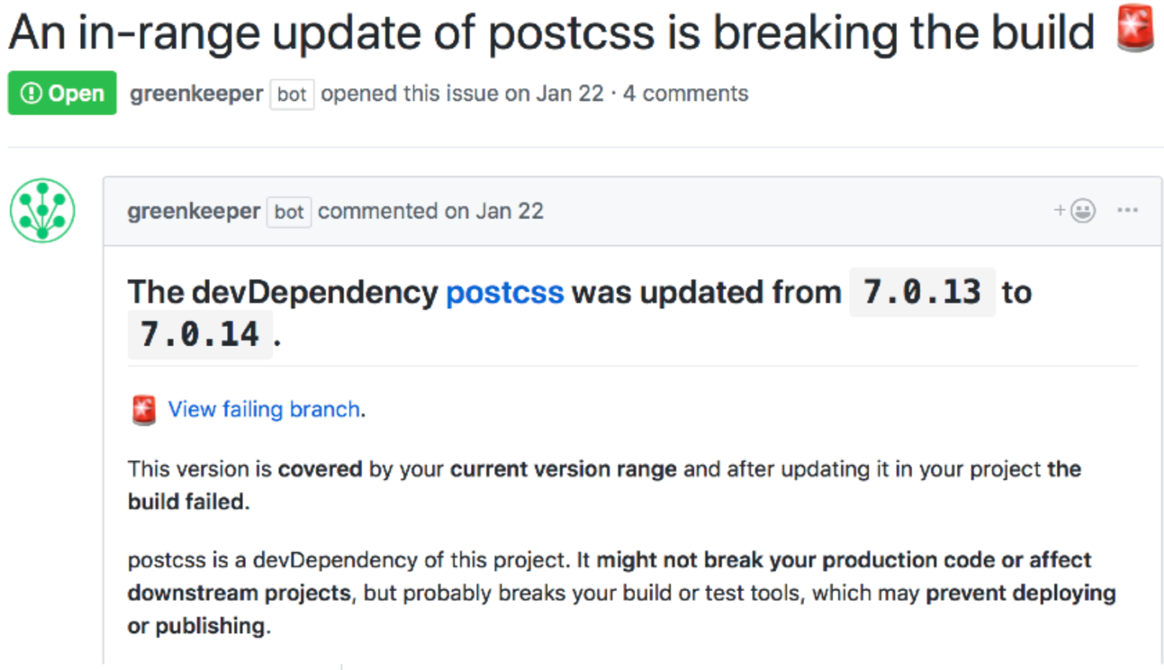
\includegraphics[width=8cm]{images/gk_issue.png}
    \caption{A Greenkeeper in-range issue report}
    \label{fig:gk_issue_report}
\end{figure}
\par
An in-range update means that a client will accept the update without having to change their version specification. For example, If a client specifies an accepted version range of $\string^$1.0.0 for a dependency, and that dependency releases version 1.0.1, that update is in-range. Users of the client's package would receive this update when they run \textit{npm install}. If an update is out of range of a client's version specification, they will not receive the update. So if an an out-of-range update breaks a client, their user's will not be effected. 



